% Options for packages loaded elsewhere
\PassOptionsToPackage{unicode}{hyperref}
\PassOptionsToPackage{hyphens}{url}
%
\documentclass[
]{book}
\usepackage{amsmath,amssymb}
\usepackage{iftex}
\ifPDFTeX
  \usepackage[T1]{fontenc}
  \usepackage[utf8]{inputenc}
  \usepackage{textcomp} % provide euro and other symbols
\else % if luatex or xetex
  \usepackage{unicode-math} % this also loads fontspec
  \defaultfontfeatures{Scale=MatchLowercase}
  \defaultfontfeatures[\rmfamily]{Ligatures=TeX,Scale=1}
\fi
\usepackage{lmodern}
\ifPDFTeX\else
  % xetex/luatex font selection
\fi
% Use upquote if available, for straight quotes in verbatim environments
\IfFileExists{upquote.sty}{\usepackage{upquote}}{}
\IfFileExists{microtype.sty}{% use microtype if available
  \usepackage[]{microtype}
  \UseMicrotypeSet[protrusion]{basicmath} % disable protrusion for tt fonts
}{}
\makeatletter
\@ifundefined{KOMAClassName}{% if non-KOMA class
  \IfFileExists{parskip.sty}{%
    \usepackage{parskip}
  }{% else
    \setlength{\parindent}{0pt}
    \setlength{\parskip}{6pt plus 2pt minus 1pt}}
}{% if KOMA class
  \KOMAoptions{parskip=half}}
\makeatother
\usepackage{xcolor}
\usepackage{color}
\usepackage{fancyvrb}
\newcommand{\VerbBar}{|}
\newcommand{\VERB}{\Verb[commandchars=\\\{\}]}
\DefineVerbatimEnvironment{Highlighting}{Verbatim}{commandchars=\\\{\}}
% Add ',fontsize=\small' for more characters per line
\usepackage{framed}
\definecolor{shadecolor}{RGB}{248,248,248}
\newenvironment{Shaded}{\begin{snugshade}}{\end{snugshade}}
\newcommand{\AlertTok}[1]{\textcolor[rgb]{0.94,0.16,0.16}{#1}}
\newcommand{\AnnotationTok}[1]{\textcolor[rgb]{0.56,0.35,0.01}{\textbf{\textit{#1}}}}
\newcommand{\AttributeTok}[1]{\textcolor[rgb]{0.13,0.29,0.53}{#1}}
\newcommand{\BaseNTok}[1]{\textcolor[rgb]{0.00,0.00,0.81}{#1}}
\newcommand{\BuiltInTok}[1]{#1}
\newcommand{\CharTok}[1]{\textcolor[rgb]{0.31,0.60,0.02}{#1}}
\newcommand{\CommentTok}[1]{\textcolor[rgb]{0.56,0.35,0.01}{\textit{#1}}}
\newcommand{\CommentVarTok}[1]{\textcolor[rgb]{0.56,0.35,0.01}{\textbf{\textit{#1}}}}
\newcommand{\ConstantTok}[1]{\textcolor[rgb]{0.56,0.35,0.01}{#1}}
\newcommand{\ControlFlowTok}[1]{\textcolor[rgb]{0.13,0.29,0.53}{\textbf{#1}}}
\newcommand{\DataTypeTok}[1]{\textcolor[rgb]{0.13,0.29,0.53}{#1}}
\newcommand{\DecValTok}[1]{\textcolor[rgb]{0.00,0.00,0.81}{#1}}
\newcommand{\DocumentationTok}[1]{\textcolor[rgb]{0.56,0.35,0.01}{\textbf{\textit{#1}}}}
\newcommand{\ErrorTok}[1]{\textcolor[rgb]{0.64,0.00,0.00}{\textbf{#1}}}
\newcommand{\ExtensionTok}[1]{#1}
\newcommand{\FloatTok}[1]{\textcolor[rgb]{0.00,0.00,0.81}{#1}}
\newcommand{\FunctionTok}[1]{\textcolor[rgb]{0.13,0.29,0.53}{\textbf{#1}}}
\newcommand{\ImportTok}[1]{#1}
\newcommand{\InformationTok}[1]{\textcolor[rgb]{0.56,0.35,0.01}{\textbf{\textit{#1}}}}
\newcommand{\KeywordTok}[1]{\textcolor[rgb]{0.13,0.29,0.53}{\textbf{#1}}}
\newcommand{\NormalTok}[1]{#1}
\newcommand{\OperatorTok}[1]{\textcolor[rgb]{0.81,0.36,0.00}{\textbf{#1}}}
\newcommand{\OtherTok}[1]{\textcolor[rgb]{0.56,0.35,0.01}{#1}}
\newcommand{\PreprocessorTok}[1]{\textcolor[rgb]{0.56,0.35,0.01}{\textit{#1}}}
\newcommand{\RegionMarkerTok}[1]{#1}
\newcommand{\SpecialCharTok}[1]{\textcolor[rgb]{0.81,0.36,0.00}{\textbf{#1}}}
\newcommand{\SpecialStringTok}[1]{\textcolor[rgb]{0.31,0.60,0.02}{#1}}
\newcommand{\StringTok}[1]{\textcolor[rgb]{0.31,0.60,0.02}{#1}}
\newcommand{\VariableTok}[1]{\textcolor[rgb]{0.00,0.00,0.00}{#1}}
\newcommand{\VerbatimStringTok}[1]{\textcolor[rgb]{0.31,0.60,0.02}{#1}}
\newcommand{\WarningTok}[1]{\textcolor[rgb]{0.56,0.35,0.01}{\textbf{\textit{#1}}}}
\usepackage{longtable,booktabs,array}
\usepackage{calc} % for calculating minipage widths
% Correct order of tables after \paragraph or \subparagraph
\usepackage{etoolbox}
\makeatletter
\patchcmd\longtable{\par}{\if@noskipsec\mbox{}\fi\par}{}{}
\makeatother
% Allow footnotes in longtable head/foot
\IfFileExists{footnotehyper.sty}{\usepackage{footnotehyper}}{\usepackage{footnote}}
\makesavenoteenv{longtable}
\usepackage{graphicx}
\makeatletter
\def\maxwidth{\ifdim\Gin@nat@width>\linewidth\linewidth\else\Gin@nat@width\fi}
\def\maxheight{\ifdim\Gin@nat@height>\textheight\textheight\else\Gin@nat@height\fi}
\makeatother
% Scale images if necessary, so that they will not overflow the page
% margins by default, and it is still possible to overwrite the defaults
% using explicit options in \includegraphics[width, height, ...]{}
\setkeys{Gin}{width=\maxwidth,height=\maxheight,keepaspectratio}
% Set default figure placement to htbp
\makeatletter
\def\fps@figure{htbp}
\makeatother
\setlength{\emergencystretch}{3em} % prevent overfull lines
\providecommand{\tightlist}{%
  \setlength{\itemsep}{0pt}\setlength{\parskip}{0pt}}
\setcounter{secnumdepth}{5}
\usepackage{booktabs}
\ifLuaTeX
  \usepackage{selnolig}  % disable illegal ligatures
\fi
\usepackage[]{natbib}
\bibliographystyle{plainnat}
\IfFileExists{bookmark.sty}{\usepackage{bookmark}}{\usepackage{hyperref}}
\IfFileExists{xurl.sty}{\usepackage{xurl}}{} % add URL line breaks if available
\urlstyle{same}
\hypersetup{
  pdftitle={docs.audioblast.org},
  pdfauthor={Ed Baker},
  hidelinks,
  pdfcreator={LaTeX via pandoc}}

\title{docs.audioblast.org}
\author{Ed Baker}
\date{2024-01-12}

\begin{document}
\maketitle

{
\setcounter{tocdepth}{1}
\tableofcontents
}
\hypertarget{about-audioblast}{%
\chapter{About audioBlast}\label{about-audioblast}}

audioBlast is a project to make the world's collections of bioacoustic and ecoacoustic recordings findable, accessible, and searchable.

\hypertarget{introduction}{%
\chapter{Introduction}\label{introduction}}

\hypertarget{design-philosophy}{%
\section{Design Philosophy}\label{design-philosophy}}

The technical design of audioBlast pushes computation down the stack as far as is conveniently possible. Ideally this will often be the database. This results in a reduction in network traffic, which can be significant if returning a large number of analyses.

Some core parts of the audioBlast system (i.e.~the ingest process and analyse process) can communicate directly with the database, and all insertion or updating of records must be performed through one of these processes.

In general, and for all end-user cases, reading of data should be performed via the API (\url{https://api.audioblast.org}). The API is a lightweight database wrapper that automatically handles pagination of results and caching of slow queries. Various utilities provide access to the API in different environments, including the sonicscrewdriver package for the R environment. The API is also used to provide the data search and discovery tools at \url{https://audioblast.org}.

\begin{table}

\caption{\label{tab:unnamed-chunk-1}Simplified illustration of audioBlast abstraction layers from 
  bottom to top.}
\centering
\begin{tabular}[t]{llll}
\toprule
  & Ingest & Analyse & API\\
\midrule
MySQL & Triggers<br><br>INSERT<br><br>UPDATE & Stored Procedures<br><br>INSERT<br><br>UPDATE & SELECT\\
R & r-dbi<br><br>abdb & r-dbi<br><br>abdb & \\
API &  &  & API QueryBuilder\\
Users &  &  & API Calls\\
\bottomrule
\end{tabular}
\end{table}

\hypertarget{analyse-everything-once-in-advance}{%
\section{Analyse everything once, in advance}\label{analyse-everything-once-in-advance}}

Many bioacoustic and ecoacoustic studies make use of a standard set of analyses. These are computed in advance by audioBlast, allowing the analyses to be instantly available and searchable. An additional advantage is that the computational resource needed to compute analyses need only be performed once.

\hypertarget{infrastructure}{%
\section{Infrastructure}\label{infrastructure}}

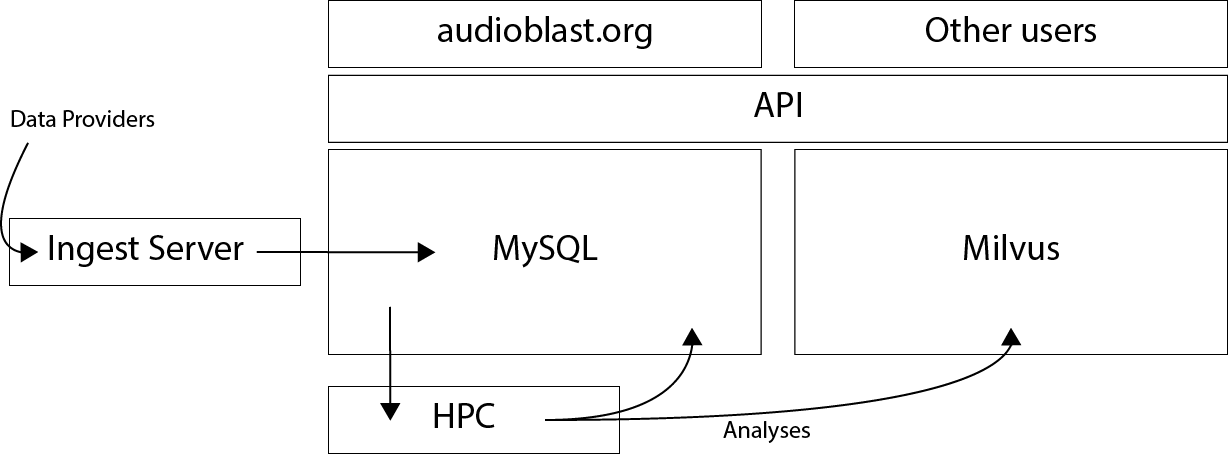
\includegraphics{images/infrastructure.png}

\hypertarget{audioblastingest}{%
\chapter{audioBlastIngest}\label{audioblastingest}}

The ingest service is responsible for bringing data about recordings, deployments, annotation, taxa and traits into the audioBlast system. Data sources are specified as modules within the audioBlast API, which give details of each data source and the processing that is expected to be performed by the ingest process. The ingest process itself is managed on audioBlast infrastructure by the audioBlastIngest package. This package obtains data from the sources specified in the API modules, performs and requested transformations, and loads the data into the audioBlast database.

Note: The database generates analysis tasks using triggers as data is inserted or updated, however the analyses are performed by a separate processes to the ingest.

Updates are handled periodically (generally nightly) by the ingest server. Creating an ingest task is a simple three step process.

\begin{enumerate}
\def\labelenumi{\arabic{enumi}.}
\item
  Third party publishes data online.
\item
  audioBlast team work with third party to create an API module to map the published data on to audioBlast data structures.
\item
  The audioBlastIngest package handles the import of the data.
\end{enumerate}

\hypertarget{source-modules}{%
\section{Source modules}\label{source-modules}}

\hypertarget{fields}{%
\subsection{Fields}\label{fields}}

\hypertarget{mapping-columns}{%
\subsection{Mapping columns}\label{mapping-columns}}

\hypertarget{optional-processing-done-by-audioblast}{%
\subsubsection{Optional processing done by audioBlast}\label{optional-processing-done-by-audioblast}}

\hypertarget{specifying-processors}{%
\paragraph{Specifying processors}\label{specifying-processors}}

\hypertarget{sourcer-automatically-prepend-a-source-column}{%
\subparagraph{SourceR: Automatically prepend a source column}\label{sourcer-automatically-prepend-a-source-column}}

\hypertarget{date2dateantime-date-and-time-mapping}{%
\subparagraph{date2dateAnTime(): Date and time mapping}\label{date2dateantime-date-and-time-mapping}}

You can map datetime fields to Date and use the date2dateAndTime() processor to split them into separate date and time fields.

\hypertarget{audioblastanalyse}{%
\chapter{audioBlastAnalyse}\label{audioblastanalyse}}

audioBlastAnalyse is an R package that handles the analysis of recordings. While some analyses (e.g.~annotations) can be imported during the ingest process this is not true for all sources of recordings.

\hypertarget{requirements}{%
\section{Requirements}\label{requirements}}

The analysis system requires a computer running the R environment for statistical computing. The package will import all dependencies on installation.

The package is tested on recent MacOS, Linux, and Windows systems.

If the analysis system is to write directly to the audioBlast database then it must additionally be on the NHM network (including via the VPN).

\hypertarget{development}{%
\section{Development}\label{development}}

The package is hosted on the audioBlast GitHub at \url{https://github.com/audioblast/audioBlastAnalyse}.

\hypertarget{installation}{%
\section{Installation}\label{installation}}

Installation of the package requires the devtools package.

\begin{Shaded}
\begin{Highlighting}[]
\FunctionTok{install.packages}\NormalTok{(}\StringTok{"devtools"}\NormalTok{)}
\end{Highlighting}
\end{Shaded}

\hypertarget{from-github}{%
\subsection{From GitHub}\label{from-github}}

\begin{Shaded}
\begin{Highlighting}[]
\NormalTok{devtools}\SpecialCharTok{::}\FunctionTok{install\_github}\NormalTok{(}\StringTok{"audioblast/audioBlastAnalyse"}\NormalTok{)}
\end{Highlighting}
\end{Shaded}

\hypertarget{from-r-working-directory}{%
\subsection{From R working directory}\label{from-r-working-directory}}

\begin{Shaded}
\begin{Highlighting}[]
\NormalTok{devtools}\SpecialCharTok{::}\FunctionTok{install}\NormalTok{()}
\end{Highlighting}
\end{Shaded}

\hypertarget{adding-new-analyses}{%
\chapter{Adding new analyses}\label{adding-new-analyses}}

The process for adding new analyses is:

\begin{enumerate}
\def\labelenumi{\arabic{enumi}.}
\item
  Create a new database table for storing the analysis, following the column tyes and names of `analysis-aci'.
\item
  Add the analysis table to the deleteAllAnalyses() function of audioBlastAnalyse R package.
\item
  Implement the analysis in audioBlastAnalyse R package.
\item
  Implement a module for \url{https://api.audioblast.org} to provide API access to the analysis.
\item
  Make arrangements for existing recordings to be queued for analysis if required.
\end{enumerate}

\hypertarget{the-task-queue-system}{%
\chapter{The Task Queue System}\label{the-task-queue-system}}

The Task Queue System maintains a list of outstanding analysis tasks in the database and is responsible for assigning tasks to analysis processes.

The database implementation is designed so that it can be utilised by either audioBlastAnalyse or in the future by an analysis package in another language (e.g.~a Python analysis suite).

\hypertarget{database-implementation}{%
\section{Database Implementation}\label{database-implementation}}

The system is implemented as two tables in the database, \texttt{tasks} and \texttt{tasks-progress}. Tasks are assigned using the stored procedure \texttt{get-tasks()} for local files, or \texttt{get-tasks-by-file()} for web files. The \texttt{get-tasks()} procedure will assign \texttt{n} random tasks to the analysis process, whereas \texttt{get-tasks-by-file()} will return all outstanding tasks for a given file. The latter procedure removes the need for repeated downloads of the same file.

\hypertarget{tasks-table}{%
\subsection{\texorpdfstring{\texttt{tasks} table}{tasks table}}\label{tasks-table}}

The table \texttt{tasks} is a list of outstanding analysis tasks. It is populated automatically by triggers on the \texttt{recordings} and \texttt{recordings-calcuated} table. Analysis tasks are grouped into sections (recordings\_calculated, sounscapes\_minute and soundscpaes\_second). The \texttt{recordings-calculaed} table has a TINYINT column for each of these, that is set to \texttt{1} once the task is completed.

\hypertarget{tasks-progress-table}{%
\subsection{\texorpdfstring{\texttt{tasks-progress} table}{tasks-progress table}}\label{tasks-progress-table}}

The table \texttt{tasks-progress} is populated by the stored procedure \texttt{get-tasks()} when an analysis process requests outstanding tasks. It is used to prevent the same task being analysed to multiple analysis processes. Tasks from an unresponsive process (e.g.~a process which has crashed) can be reassigned after an hour of inactivity by that process.

\hypertarget{get-tasks-stored-procedure}{%
\subsection{\texorpdfstring{\texttt{get-tasks()} stored procedure}{get-tasks() stored procedure}}\label{get-tasks-stored-procedure}}

The stored procedure \texttt{get-tasks(process\_id,\ n,\ source)} is used to assign \texttt{n} tasks to the analysis process \texttt{process\_id}. Initially a call to \texttt{\_quickMaintain()} is performed to deallocate time-expired tasks. It inserts \texttt{n} random unassigned tasks from the \texttt{tasks} table into the \texttt{tasks-progress} table along with the process\_id and the current timestamp. It returns via a SELECT statement these tasks.

\hypertarget{get-tasks-by-file-stored-procedure}{%
\subsection{\texorpdfstring{\texttt{get-tasks-by-file()} stored procedure}{get-tasks-by-file() stored procedure}}\label{get-tasks-by-file-stored-procedure}}

Initially a call to \texttt{\_quickMaintain()} is performed to deallocate time-expired tasks. The stored procedure \texttt{get-tasks(process\_id,\ source)} then assigns all outstanding tasks for a randomly chosen file to the analysis process \texttt{process\_id}. It inserts these tasks from the \texttt{tasks} table into the \texttt{tasks-progress} table along with the process\_id and the current timestamp. It returns via a SELECT statement these tasks.

\hypertarget{delete-task-stored-proecure}{%
\subsection{\texorpdfstring{\texttt{delete-task()} stored proecure}{delete-task() stored proecure}}\label{delete-task-stored-proecure}}

The stored procedure \texttt{delete-task(process\_id,\ source,\ id,\ task)} marks a task as complete by deleting it from the \texttt{tasks} table. A trigger in the \texttt{tasks} table will delete the matching row from \texttt{tasks-progress}. The started time of any remaining tasks assigned to the same \texttt{process\_id} in the \texttt{tasks-progess} table will be updated to the current time. A call is made to the stored procedure \texttt{\_quickMaintain()} which will perform routine maintenance tasks, including removing any expired tasks in the \texttt{tasks-progress} table.

\hypertarget{audioblastanalyse-implementation}{%
\section{audioBlastAnalyse Implementation}\label{audioblastanalyse-implementation}}

The analysis suite audioBlastAnalyse has several functions that implement this task queue in the R language.

All these functions require a database connector (\texttt{db}) as a parameter, and a unique \texttt{process\_id} for the analysis process. In the majority of cases these functions will be called automatically from within a call to the main \texttt{analyse()} function, where the database connector will already be configured and a process identifier is automatically generated.

\hypertarget{legacy-mode}{%
\subsection{Legacy mode}\label{legacy-mode}}

On some older Linux operating systems the RMariaDB package and libraries it builds against have issues dealing with stored procedures. For the time being a legacy mode is provided that implements the stored procedures as a sequence of queries. Setting \texttt{legacy=TRUE} as a parameter to either of the fetch queries will activate this mode.

\hypertarget{getting-tasks}{%
\subsection{Getting tasks}\label{getting-tasks}}

The \texttt{get-tasks()} stored procedure is accessed by using \texttt{fetchDownloadableRecordings()}, and \texttt{get-tasks-by-file()} by using \texttt{fetchDownloadableRecordings()}.

\begin{Shaded}
\begin{Highlighting}[]
\FunctionTok{fetchDownloadableRecordings}\NormalTok{(db, source, process\_id, }\AttributeTok{legacy=}\ConstantTok{FALSE}\NormalTok{)}
\FunctionTok{fetchUnanalysedRecordings}\NormalTok{(db, source, process\_id, }\AttributeTok{legacy=}\ConstantTok{FALSE}\NormalTok{)}
\end{Highlighting}
\end{Shaded}

\hypertarget{removing-completed-tasks}{%
\subsection{Removing completed tasks}\label{removing-completed-tasks}}

\begin{Shaded}
\begin{Highlighting}[]
\FunctionTok{deleteToDo}\NormalTok{(db, source, id, task, process\_id)}
\end{Highlighting}
\end{Shaded}

\hypertarget{analysis-infrastructure}{%
\chapter{Analysis infrastructure}\label{analysis-infrastructure}}

\hypertarget{natural-history-museum-high-performance-compute}{%
\section{Natural History Museum High-Performance Compute}\label{natural-history-museum-high-performance-compute}}

The Natural History Museum has a high-performance compute cluster that can be used for audio analysis. The cluster is managed using SLURM and environments are managed using conda.

\hypertarget{conda-environments}{%
\subsection{conda environments}\label{conda-environments}}

\hypertarget{ab-r2}{%
\subsubsection{ab-r2}\label{ab-r2}}

This environment contains R packages for acoustic analysis, and also has audioBlastAnalyse installed to manage analyses.

\begin{Shaded}
\begin{Highlighting}[]
\ExtensionTok{conda}\NormalTok{ activate ab{-}r2}
\end{Highlighting}
\end{Shaded}

\hypertarget{birdnet}{%
\subsubsection{birdnet}\label{birdnet}}

This is a Python environment for running BirdNET analyses.

\begin{Shaded}
\begin{Highlighting}[]
\ExtensionTok{conda}\NormalTok{ activate birdnet}
\end{Highlighting}
\end{Shaded}

\hypertarget{audioblast.org}{%
\chapter{audioblast.org}\label{audioblast.org}}

The website provides a convenient search and browsing interface making use of api.audioblast.org. This server is hosted by the Natural History Museum, London.

\hypertarget{search-module-api}{%
\chapter{Search module API}\label{search-module-api}}

The search module API allows for processing of a search term on audioblast.org, and handles the display of relevant search results. Modules are typically related to a particular data type (i.e.~a table in the audioblast database), although there are more abstract modules that solely process search terms in order to allow them to be processed by other modules.

\hypertarget{search-api-class}{%
\section{Search API class}\label{search-api-class}}

\hypertarget{init}{%
\subsection{init()}\label{init}}

\hypertarget{displayprototype}{%
\subsection{displayPrototype()}\label{displayprototype}}

Create a region on the results page for displaying search results.

\hypertarget{parse}{%
\subsection{parse()}\label{parse}}

Parses the search term for relevant terms, and may modify terms.

\hypertarget{display}{%
\subsection{display()}\label{display}}

Handles the display of search results to the user.

\hypertarget{searchsuggests}{%
\subsection{searchSuggests()}\label{searchsuggests}}

Provides a short list of indicative search terms that may be handled by the module. This is used to suggest search terms on the audioblast.org homepage.

\hypertarget{current-audioblast.org-search-modules}{%
\section{Current audioblast.org search modules}\label{current-audioblast.org-search-modules}}

\hypertarget{pythia}{%
\subsection{Pythia}\label{pythia}}

Pythia uses an audioBlast API to match words in the search term to tokens using direct access to the audioBlast database.

\hypertarget{linnaeus-taxonomic-name-information-and-processing}{%
\subsection{Linnaeus: taxonomic name information and processing}\label{linnaeus-taxonomic-name-information-and-processing}}

The parse() function in Linnaeus takes a taxon name token identified by Pythia and converts it to a taxon name with rank token.

Linnaeus also handles the taxon info box, that provides search navigation through parent taxa.

\hypertarget{king-solomons-ring}{%
\subsection{King Solomon's Ring}\label{king-solomons-ring}}

King Solomon's Ring converts everyday terms relating to animal behavior into named trait with value tokens (e.g.~silent to sound production method being equal to None.)

\hypertarget{rosetta}{%
\subsection{Rosetta}\label{rosetta}}

Rosetta handles the conversion of emoji in search terms to taxonomic names using the Phymoji package.

\hypertarget{maintenence-tasks}{%
\chapter{Maintenence tasks}\label{maintenence-tasks}}

\hypertarget{cron-tasks}{%
\section{cron tasks}\label{cron-tasks}}

Every 5 minutes a cron job on the unp-audio-2 virtual machine updates the total analysis counts by calling the API endpoint /standalone/analysis/fetch\_analysis\_counts/ without caching (?cache=0).

Other slow-running queries that impact the speed of the user interface can be added here if necessary.

\hypertarget{maintenence-notices}{%
\chapter{Maintenence notices}\label{maintenence-notices}}

These are created and displayed on the status.acousti.cloud server, at present by directly editing the table notices in the status MySQL database. The active column is set to 1 for active notices.

  \bibliography{book.bib,packages.bib}

\end{document}
